\documentclass[conference]{IEEEtran}

\input{includes/preamble_common}
% Bibliografía para IEEE (usando BibTeX)
\usepackage{natbib}

% Keywords helper
\providecommand{\keywords}[1]{\textbf{Palabras clave: } #1}

\begin{document}

\title{Articulo de investigación SchoolMe }

\author{
\IEEEauthorblockN{Jesus Fernando Carvajal Anacona\IEEEauthorrefmark{1}}
\IEEEauthorblockA{\IEEEauthorrefmark{1}Afiliación 1, Neiva, Colombia — \texttt{jesusanacona017@gmail.com}}
% \IEEEauthorblockA{\IEEEauthorrefmark{2}Afiliación 2, Ciudad, País — \texttt{autor2@ejemplo.edu}}
}

\maketitle

\begin{abstract}
Las metodologías ágiles han mejorado el desarrollo de software gracias a la adaptabilidad, colaboración y entrega continua de valor. En este artículo se analizan las distintas investigaciones sobre la aplicación de estas metodologías en la gestión de proyectos empresariales y tecnológicos
Estas metodologías están representadas principalmente por Scrum y Kanban, emergen como marcos que le han dado un nuevo significado a la forma de planificar, ejecutar y evaluar proyectos, permiten ciclos de entrega más cortos y un enfoque orientado al cliente, estos enfoques han superado progresivamente a los modelos tradicionales como Waterfall, cuya rigidez ha evidenciado limitaciones en contextos donde la flexibilidad es indispensable.

Dentro de las investigaciones analizadas sobresale el papel de Scrum como metodología predominante en proyectos empresariales y académicos. Su estructura basada en sprints, reuniones iterativas y roles definidos como el Product Owner, el Scrum Master y el Development Team ha permitido fortalecer la comunicación, mantener ciclos constantes de retroalimentación y garantizar un avance progresivo incluso en escenarios complejos. Sin embargo, la efectividad de Scrum no depende únicamente de su concepto, sino también del comportamiento, comunicación transversal, liderazgo y adaptabilidad cultural. Esto se deja claro en investigaciones sobre desarrollo global (GSD), donde los equipos distribuidos geográficamente enfrentan retos de zona horaria, barreras lingüísticas y diferencias organizacionales. En estos contextos, la metodología demuestra ser eficiente, siempre y cuando exista un liderazgo capaz de ordenar la colaboración remota y sostener la cohesión del equipo.

Del mismo modo, los estudios sobre diversidad de género revelan que la dinámica colaborativa también está profundamente influida por factores sociales. Los equipos con composición equilibrada entre hombres y mujeres presentan mejores resultados en diseño, calidad de trabajo y organización. Estos hallazgos muestran que la agilidad no se limita al uso de herramientas o prácticas técnicas, sino que implica una comprensión de la forma en cómo se relacionan las personas, la distribución de tareas y la percepción del rol individual dentro del grupo. Este componente social, muchas veces ignorado en la ingeniería de software tradicional, se convierte en un factor importante para determinar la calidad y la velocidad de entrega.

Otro punto a tomar en cuenta es el análisis de la aplicación diferenciada de metodologías ágiles según el ecosistema tecnológico. El contraste entre desarrollos para iOS y Android evidencia que, aunque ambos entornos pueden beneficiarse de Scrum y Kanban, presentan características propias que modifican tiempos, pruebas y niveles de exigencia. En iOS, la uniformidad del hardware acelera la validación, mientras que la diversidad de dispositivos Android hace más lento el proceso pero amplía los escenarios de prueba. Estos resultados resaltan que la agilidad no debe aplicarse como una fórmula absoluta, sino como un conjunto adaptable de principios capaces de ajustarse a las necesidades específicas de cada proyecto y plataforma.

La unión entre Agile, DevOps y tecnologías en la nube representa una de las transformaciones más relevantes del panorama actual. La integración entre estos enfoques permite automatizar despliegues, optimizar recursos y aumentar la frecuencia de entregas sin comprometer la calidad. No obstante, este modelo también enfrenta desafíos relacionados con la complejidad técnica, la proliferación de herramientas, las competencias requeridas en los equipos y la necesidad de garantizar seguridad en cada etapa del ciclo de vida del software. De ahí la relevancia de DevSecOps, que incorpora prácticas de ciberseguridad dentro de los sprints, automatiza pruebas de seguridad en pipelines CI/CD y redefine la forma en que se gestionan riesgos en sistemas ágiles. Esta integración es clave para lograr productos grandes capaces de resistir el aumento de amenazas, vulnerabilidades y ataques sofisticados.

Se observa una tendencia hacia modelos híbridos que combinan Agile con enfoques tradicionales o con marcos de mejora continua como Lean Six Sigma. Esta integración permite equilibrar agilidad con precisión analítica, adaptabilidad con eficiencia operativa y velocidad con control. Los estudios evidencian que estos enfoques híbridos reducen defectos, optimizan tiempos y refuerzan la toma de decisiones basada en datos. Sin embargo, requieren liderazgo sólido, capacitación constante y una adecuada cultura organizacional para evitar conflictos entre los principios de cada metodología.

Una contribución destacada es el análisis de la calidad de los requisitos, uno de los aspectos más críticos en la ingeniería de software. La comparación entre documentación convencional y documentación en pares revela que la segunda produce especificaciones más completas, consistentes y menos ambiguas. La colaboración directa evita interpretaciones equivocadas, identifica omisiones y hace que el documento evolucione de manera coherente con el proyecto. Esto demuestra que incluso en entornos ágiles, donde la documentación suele ser mínima, la calidad del SRS sigue siendo esencial para evitar sobrecostos, retrasos y fallos en el producto final.

Se explora la innovación mediante lógica difusa para medir el nivel de agilidad real en los equipos. Este modelo permite traducir percepciones subjetivas en métricas objetivas, generando un sistema capaz de evaluar la madurez ágil con precisión y sin depender exclusivamente de indicadores parciales. La introducción de inteligencia artificial en la medición de prácticas ágiles constituye un avance significativo para organizaciones que buscan monitorear su evolución y detectar oportunidades de mejora.

Respecto al aseguramiento de calidad, los estudios sobre automatización de pruebas y optimización de pipelines CI/CD muestran cómo la velocidad del desarrollo moderno exige herramientas que reduzcan el esfuerzo manual, mejoren la estabilidad y eviten errores en producción. Automatizar pruebas E2E con Selenium, por ejemplo, ha demostrado ser fundamental para garantizar flujos críticos en sistemas de comercio electrónico. Al mismo tiempo, optimizar pipelines CI/CD mediante paralelización, análisis de métricas y entornos consistentes responde a la necesidad de entregas más confiables sin sacrificar la rapidez. Esto confirma que la automatización dejó de ser una ventaja competitiva para convertirse en una necesidad estratégica.

La investigación aborda el enfoque emergente conocido como Algorithm-driven Development (ADD), un modelo visual que convierte los requisitos en diagramas de flujo desde el inicio del proyecto y permite detectar errores antes de escribir el código. Este método ofrece una alternativa eficiente en proyectos grandes y complejos, donde TDD o BDD pueden fallar por restricciones de tiempo o volumen de trabajo. ADD fortalece la claridad lógica del sistema y reduce defectos de forma temprana, dejando ver una evolución en la forma de concebir la ingeniería de software.

Se destaca una tendencia transversal que recorre todos los estudios: el desarrollo sostenible del software. Esto implica no solo eficiencia técnica, sino prácticas que garanticen continuidad, seguridad integrada, documentación viva, equipos capacitados y procesos capaces de adaptarse a entornos cada vez más cambiantes. Las metodologías ágiles e híbridas adquieren un papel central en esta sostenibilidad, pues permiten iterar sin sacrificar calidad y anticiparse a las necesidades del cliente y del mercado.

Las investigaciones analizadas muestran que la agilidad ha dejado de ser un conjunto de prácticas para convertirse en una filosofía organizacional que permea tecnologías, personas, herramientas y comportamientos. Su éxito radica en la capacidad de integrar colaboración, automatización, liderazgo, seguridad y experimentación constante. Más que acelerar procesos, la agilidad cambia la manera en la que los equipos conciben el trabajo, enfrentan la incertidumbre y crean soluciones. 



\end{abstract}

\begin{IEEEkeywords}
buenas prácticas, ingeniería de software, investigación aplicada, reproducibilidad
\end{IEEEkeywords}

\section{Introducción}
La industria del software demanda calidad, rapidez y sostenibilidad. Las \textit{buenas prácticas} como control de versiones, integración continua \cite{fowler2006continuous}, desarrollo dirigido por pruebas \cite{beck2003testdriven}, y entrega continua \cite{chen2015devops} prometen mejorar resultados, pero su efectividad varía según contexto. 

Este trabajo investiga, de forma aplicada, cómo un conjunto curado de prácticas influye en resultados verificables y en la construcción de un \textit{software funcional}. Siguiendo los principios de código limpio \cite{martin2008clean} y las métricas DORA \cite{dora2021metrics}, evaluamos el impacto de estas prácticas en un proyecto real.

Nuestras contribuciones son: (1) un protocolo reproducible para aplicar y medir prácticas, (2) un estudio con métricas de proceso y producto basado en \cite{forsgren2018accelerate}, y (3) una guía de lecciones aprendidas para la industria.
\section{Estado del Arte Humanizado: Convergencia de Bienestar, Rigor y Ética}
El estado del arte revela que la relación entre la innovación tecnológica y el desarrollo humano ha sido abordada desde múltiples ángulos disciplinarios, todos los cuales convergen en la necesidad de equilibrar el potencial de la tecnología con el bienestar, el rigor y la ética. Esta revisión, fundamentada en diecisiete estudios, permite identificar patrones consistentes en torno a las vulnerabilidades humanas y metodológicas en el ecosistema digital.

I. El Factor Humano: Vulnerabilidades y Alfabetización Digital
La literatura especializada demuestra que la eficacia de los sistemas avanzados a menudo está limitada por el comportamiento y las capacidades biológicas del usuario.

Riesgo en Ciberseguridad y Comportamiento: En el campo de la ciberseguridad móvil, investigaciones como las de Prieto et al. \cite{Prieto2018} indican que el usuario suele subestimar la importancia de los permisos en sistemas operativos como Android. Este factor no es primordialmente técnico, sino un asunto de alfabetización digital y comportamiento, abriendo puertas a un creciente número de ataques y fugas de datos.

Ergonomía y Salud Visual (SVI): La exposición prolongada a pantallas ha generado problemas de salud ocupacional de creciente relevancia. Frometa et al. \cite{Frometa2012} y Miró \cite{Miro2005} evidencian que el Síndrome Visual Informático (SVI), junto a la fatiga cognitiva derivada de la privación de sueño, no solo afecta la visión, sino que disminuye el rendimiento cognitivo y la estabilidad emocional. Esto transforma la mala gestión tecnológica en un factor de deterioro silencioso con impacto directo en la productividad y la calidad de vida.

Inclusión y Adaptabilidad: En el diseño de software, la dimensión humana se extiende a la inclusión. Estudios como los de Pacheco et al. \cite{Pacheco2020} sobre software inclusivo para niños con Síndrome de Down leve demuestran que las decisiones de diseño tienen un impacto directo en las oportunidades de aprendizaje y la integración social, resaltando que el diseño ético debe ser fundamentalmente adaptativo.

II. Rigor Metodológico y Estandarización en Ingeniería
La complejidad inherente a los gigasistemas y a la multiplicidad de opciones tecnológicas exige que las decisiones de ingeniería se basen en métricas objetivas y rigurosas.

Calidad de Software (ISO/IEC 25000): La evaluación comparativa de frameworks web, como la realizada entre Laravel y Django por Espinosa \cite{Espinosa2021} y Tolosa \cite{Tolosa2014}, subraya que la calidad del software no debe basarse en modas o preferencias subjetivas, sino en criterios verificables y estandarizados conforme a normativas internacionales como la ISO/IEC 25000.

Interoperabilidad y Continuidad del Negocio: Bishop et al. \cite{Bishop2005} abordan el desafío de integrar sistemas heredados (como Java) con soluciones modernas (C\#). La interoperabilidad se presenta como una estrategia metodológica clave para la continuidad del negocio, asegurando que los sistemas puedan convivir sin requerir migraciones costosas y disruptivas.

Automatización como Necesidad: La creciente escala y complejidad de los sistemas requiere que la Automatización de Calidad (AQ) y el uso de Inteligencia Artificial para desarrolladores \cite{Rivas2025,Gruber2024} se conviertan en mecanismos de control y reducción de riesgo sistémico \cite{Simmons2024}, dado que la supervisión humana directa ya no es viable.

III. Tecnología, Ética y Mediación Pedagógica
Más allá de lo técnico, la literatura confirma que los sistemas avanzados plantean profundas disyuntivas éticas y no pueden sustituir la intervención pedagógica humana.

Riesgos de Vigilancia y Sesgo Algorítmico: Garvie \cite{Garvie2024} aborda el uso del reconocimiento facial, destacando que el avance de la automatización y la vigilancia podría escalar sin control si no existen marcos regulatorios claros y un diseño basado en la privacidad. Los riesgos éticos no son solo técnicos, sino sociopolíticos.

IA y el Rol Humano en el Desarrollo: La integración de la IA en el ciclo de desarrollo \cite{Rivas2025} cambia el rol del programador de ejecutor a arquitecto y validador. La IA gestiona la complejidad, pero el humano mantiene el juicio ético y la creatividad final.

Software Educativo y Mediación: Los estudios en el área de la didáctica, como los de Marquès \cite{MarquesSF} y Ribas-Xirgo \cite{Ribas2008}, indican que los sistemas de acompañamiento digital y los mapas conceptuales \cite{Alaminos2009} no sustituyen el rol del educador. Por el contrario, amplifican su capacidad para orientar, clarificar y evaluar la experiencia de aprendizaje, haciendo de la mediación pedagógica un elemento indispensable para el éxito tecnológico.

Conclusión de la Revisión: El análisis demuestra que, aunque los temas son diversos, existe una unidad conceptual irrefutable: la tecnología es un espejo de las decisiones humanas. Su valor real reside en su implementación consciente, ética y rigurosa.
\section{Metodología de investigación aplicada}
Se realizó una revisión sistemática de artículos científicos publicados entre los años 2015 y 2025, seleccionados por su relevancia en el ámbito de la ingeniería de software, la gestión de proyectos y la innovación tecnológica. Las fuentes fueron obtenidas de bases de datos académicas y revistas especializadas, priorizando investigaciones indexadas y de acceso verificable. Entre ellas se encuentran Procedia Computer Science, Information and Software Technology, International Journal of Technology, Management and Humanities, World Journal of Advanced Research and Reviews e IEEE Access, entre otras \cite{Stray2025,Jain2025,PriyankaMalla2025,Solige2025,Qamar2025,ElAouni2025}.

En primer lugar, se realizó la búsqueda, selección y clasificación de los artículos según criterios temáticos: fundamentos del pensamiento ágil, estudios comparativos entre metodologías (Scrum, Kanban, Waterfall), integración con tecnologías emergentes (DevOps, Cloud, IA), gestión del riesgo, diversidad de equipos y seguridad del software \cite{William2025,LS2025,Jibgah2025,Khan2025,Ok2025}. En segundo lugar, se llevó a cabo una lectura crítica y analítica, enfocada en identificar coincidencias, diferencias y aportes relevantes entre los distintos enfoques. Finalmente, se elaboró una síntesis interpretativa que permitió articular los resultados de los estudios bajo una perspectiva integradora y contextualizada \cite{Maidin2025,JawishAlgorithm}.

\begin{figure}[h!]
    \centering
    \includegraphics[width=0.85\linewidth]{graphics/grafica2.png}
    \caption{Proceso de búsqueda, selección y clasificación de los artículos analizados.}
    \label{fig:grafica2}
\end{figure}

La investigación se apoyó en un proceso de reflexión cruzado en el que se contrastaron los hallazgos teóricos con las implicaciones prácticas descritas en los estudios. Esto permitió construir una visión global sobre la evolución de las metodologías ágiles, su impacto en la calidad, la productividad y la cultura de trabajo en entornos de desarrollo de software \cite{PriyankaMalla2025,William2025}.

La metodología se enfoca en el estudio de las investigaciones como herramienta para comprender cómo las prácticas ágiles, más allá de ser marcos técnicos, representan una transformación cultural que une tecnología, liderazgo y colaboración en la creación de soluciones digitales sostenibles \cite{LopezMenendezUnidad,Stray2025,LS2025}.

La lectura de los artículos deja claro que los temas principales son Scrum, Kanban, DevOps, nube, automatización, seguridad, híbridos ágiles, lógica difusa, colaboración, documentación, diversidad en los equipos y mejora continua \cite{Reich2025,ElAouni2025,Jibgah2025,Aguayo2025,Qamar2025}. La intención no fue clasificar los artículos de manera aislada, sino reconocer cómo cada uno aportaba una pieza al panorama general del desarrollo moderno.

Se tomó como eje común la evolución de Agile y su interacción con tecnologías y enfoques actuales. Según el análisis de las investigaciones estás se pueden conectar, por ejemplo: cómo DevOps se relaciona con automatización, cómo la documentación en pares influye en la calidad, cómo Scrum funciona en equipos distribuidos, o cómo Lean Six Sigma y Agile se complementan \cite{Reich2025,Qamar2025,Solige2025,Shriram2025,Jibgah2025}.

Después se organizaron las ideas siguiendo un hilo lógico, primero el origen de Agile y sus fundamentos; luego las adaptaciones según contexto, cultura y herramientas; después la integración con tecnologías como nube y CI/CD; y finalmente las propuestas emergentes como lógica difusa, seguridad continua e híbridos ágiles \cite{LopezMenendezUnidad,ElAouni2025,Maidin2025,Aguayo2025,Ok2025}.

El objetivo principal es guiar la adopción de agilidad dentro de organizaciones que enfrentan los equipos, demandas cambiantes, riesgos de seguridad, múltiples plataformas tecnológicas, procesos distribuidos y necesidad de automatización. La metodología se construye como un marco práctico aplicable a proyectos de cualquier tamaño, combinando principios ágiles clásicos con prácticas contemporáneas, herramientas colaborativas y estrategias de integración tecnológica \cite{Khan2025,Ok2025,Shriram2025}.

Las investigaciones dan a entender que los equipos con mayor capacidad de maniobra responden mejor a cambios repentinos. Esta flexibilidad abarca la comunicación interna, la reorganización de prioridades y la actualización de herramientas \cite{LS2025,William2025}. 

La dinámica del equipo influye directamente en la calidad del producto. Factores como diversidad de género, comunicación transversal, claridad en los roles y revisión conjunta de tareas aumentan la efectividad general \cite{Stray2025}. 

La automatización, la nube, DevOps, las pruebas continuas, la documentación colaborativa, la lógica difusa y los tableros visuales se convierten en extensiones del trabajo humano, no en sustitutos. La tecnología amplifica el rendimiento del equipo cuando se integra con propósito \cite{ElAouni2025,Maidin2025,Aguayo2025,Solige2025,Shriram2025}. 

El proceso inicia cuando el equipo adopta una preparación cultural que permite que los cambios fluyan sin resistencia. En lugar de presentar la transformación como un ajuste drástico, se introduce de manera gradual, mostrando cómo ciertas prácticas pueden resolver problemas cotidianos que antes drenaban tiempo y energía, la cultura del equipo adquiere relevancia porque influye directamente en la forma en que las personas responden ante bloqueos, revisiones y ajustes. A medida que se construye esta base cultural, el equipo define roles de manera clara, aunque sin convertirlos en barreras que limiten la interacción, cada rol funciona como una pieza que aporta una perspectiva distinta. La presencia de perfiles diversos permite enriquecer las discusiones técnicas y equilibrar la distribución de tareas, lo que disminuye la posibilidad de que ciertos integrantes carguen con responsabilidades repetitivas o poco visibles. Se sugiere que el Product Owner participe activamente en la clarificación de requisitos y en la priorización del producto para evitar interpretaciones confusas, el Scrum Master se convierte en un facilitador que garantiza que las prácticas fluyan sin interrupciones innecesarias, mientras que el equipo técnico adopta una visión amplia del trabajo para no depender de especialistas aislados. La incorporación de un Security Champion agrega una capa de protección sin frenar el avance, pues permite que la seguridad se trate como parte del desarrollo y no como un control externo que aparece al final. Esta composición diversificada no pretende crear estructuras complejas; busca que cada integrante tenga claridad sobre su aporte y que la colaboración mantenga una dirección coherente \cite{Stray2025,LS2025,Ok2025}.

Con los roles establecidos, se avanza hacia la construcción de un ciclo de trabajo que se sostenga por sí mismo, el ciclo se organiza en iteraciones que permiten retroalimentación frecuente, reducen la incertidumbre y mantienen el producto en movimiento constante, el tablero visual adquiere un papel esencial porque traduce las decisiones del equipo en una representación clara y compartida. Cada columna refleja el estado real del trabajo y permite que cualquier integrante detecte irregularidades sin necesidad de solicitudes formales, esta transparencia genera responsabilidad colectiva, reduce tiempos muertos y facilita el ajuste del trabajo cuando cambian prioridades o surge un riesgo técnico imprevisto \cite{Moiseienko2025,Reich2025}. 

La automatización temprana forma parte del ciclo desde el primer día, por eso, plantea que el equipo desarrolle pruebas unitarias, análisis estático y validaciones integrales desde la primera iteración, este enfoque no solo mejora la calidad del código, sino que también acelera la detección de problemas. El pipeline de integración continua se convierte en una herramienta que acompaña cada decisión del equipo, su función no es únicamente ejecutar pruebas, sino ofrecer información constante sobre la estabilidad del producto, cuando un error aparece, se detecta en cuestión de segundos, lo que evita que el fallo avance a etapas donde sería más costoso corregirlo. Además, el equipo aprende a interpretar los resultados del pipeline como parte de su diálogo técnico, sin que se conviertan en simples números desconectados del proceso \cite{Solige2025,Shriram2025}. 

La seguridad integrada desempeña un papel similar, no como un obstáculo externo. Esto implica revisar dependencias, analizar vulnerabilidades y evaluar riesgos desde la misma planeación del sprint, gracias a esta integración, la calidad del producto aumenta de manera orgánica, ya que los problemas de seguridad se abordan antes de que escalen. Las organizaciones que aplicaron este enfoque, según las investigaciones revisadas, lograron reducir fallos críticos sin necesidad de controles adicionales que suelen frenar el avance del desarrollo. La clave está en que la seguridad se convierte en una práctica continua, accesible para todo el equipo, y no en un control impuesto \cite{Ok2025,Khan2025}. 

La arquitectura en la nube facilita que el desarrollo mantenga consistencia, la nube permite replicar entornos sin depender de configuraciones manuales y agiliza pruebas que requieren condiciones específicas. Esta capacidad de replicación mejora la fiabilidad de las pruebas y reduce discrepancias entre ambientes, lo que se traduce en menor cantidad de errores difíciles de reproducir, los despliegues se vuelven más estables y el equipo puede experimentar con mayor libertad sin comprometer el entorno principal. Este apoyo tecnológico se integra con DevOps, que agrega prácticas de despliegue continuo y mantenimiento de entornos estables \cite{ElAouni2025,Maidin2025}. 

La documentación ocupa un lugar fundamental en esta metodología porque las investigaciones muestran que los proyectos con documentación inconsistente tienden a acumular errores, la propuesta complementaria sugiere que la documentación se construya mediante trabajo en pares, esta estrategia aumenta la claridad, evita contradicciones y mantiene la información sincronizada con el trabajo real del equipo. La creación de diagramas y representaciones visuales facilita la comprensión de la lógica del sistema y permite que las decisiones técnicas se tomen con una visión más amplia del producto, esta documentación no se trata como un requisito formal, sino como una guía que permite que todos avancen con seguridad \cite{Qamar2025,JawishAlgorithm}.



\section{Implementación: Consolidación del Modelo Teórico y Aplicabilidad Estratégica}
Dado que el presente trabajo es un artículo aplicado de revisión crítica y síntesis interpretativa, la implementación no consiste en el desarrollo de un software o un producto técnico tradicional. En cambio, su valor se materializa en la consolidación de un Modelo Teórico Holístico que traduce los hallazgos documentales en un marco conceptual coherente, útil y aplicable como base de diseño y evaluación para futuros proyectos académicos o tecnológicos.

Esta implementación se estructura en dos niveles fundamentales:

1. Integración Conceptual: El Modelo de Madurez Digital Humanizada (MMDH)
Se construyó un Modelo Interpretativo donde los diecisiete artículos revisados no se analizan de manera aislada, sino como piezas complementarias que definen un sistema de interdependencias. Este modelo permite comprender cómo interactúan y se influyen mutuamente las dimensiones críticas de cualquier desarrollo digital:

Bienestar Humano: (Ergonomía \cite{Frometa2012}, Privación del Sueño \cite{Miro2005}, Inclusión \cite{Pacheco2020}).

Calidad Tecnológica: (Rigor metodológico, Estandarización ISO/IEC 25000 \cite{Espinosa2021}, Interoperabilidad \cite{Bishop2005}).

Ética y Estrategia: (Riesgos de Vigilancia \cite{Garvie2024}, Ciberseguridad \cite{Prieto2018}, Juicio en la aplicación de IA \cite{Gruber2024}).

Este enfoque integrado permite a los investigadores y desarrolladores auditar sus proyectos bajo un único lente, reconociendo que un fallo en cualquiera de las tres dimensiones (por ejemplo, un fallo en la ergonomía) es, en esencia, un fallo en la calidad total del sistema.

2. Aplicabilidad para Futuros Proyectos: Principios Rectores
El documento final proporciona un conjunto de Principios Prácticos Rectores que orientan las decisiones técnicas y humanas en proyectos reales, asegurando que la tecnología se diseñe con conciencia estratégica. Estos principios son directamente aplicables a:

Dominio de Aplicación
Principios Prácticos Derivados

Diseño de Software Ético
Integrar el Principio de Privacidad por Defecto y realizar auditorías de Sesgo Algorítmico antes del despliegue (basado en hallazgos sobre Reconocimiento Facial \cite{Garvie2024}).

Implementación de IA Responsable
Utilizar la IA como herramienta de aumento cognitivo del desarrollador \cite{Rivas2025}, manteniendo siempre la supervisión y el juicio humano en las decisiones arquitectónicas y éticas.

Mejoras Pedagógicas basadas en TIC
Diseñar software educativo considerando la Mediación Pedagógica como un factor de éxito indispensable \cite{MarquesSF}, utilizando herramientas como los mapas conceptuales \cite{Alaminos2009} para fortalecer la comprensión significativa.

Adaptación Ergonómica y Salud
Incorporar requisitos ergonómicos y de salud visual (prevención de SVI \cite{Frometa2012}) en la fase de requisitos del software y no solo como ajustes posteriores.

Elección de Arquitecturas y Frameworks
Basar la selección tecnológica (ej., Laravel vs. Django \cite{Espinosa2021}) en Métricas de Calidad Objetivas (ISO/IEC 25000), no en preferencias subjetivas, y asegurar la interoperabilidad para la continuidad del negocio \cite{Bishop2005}.

Estrategias de Seguridad y Riesgos
Promover la formación digital del usuario para mitigar riesgos de ciberseguridad móvil \cite{Prieto2018} y establecer mecanismos de Automatización de Calidad (AQ) para reducir el riesgo sistémico en gigasistemas \cite{Simmons2024}.

De esta forma, la implementación del análisis documental se convierte en una herramienta sólida y consciente para orientar decisiones complejas en el ecosistema digital, garantizando que el diseño y la adopción tecnológica estén alineados con el bienestar humano y los estándares de calidad.
\section{Evaluación y resultados}
El análisis de las investigaciones revisadas permite comprender que la agilidad no es únicamente una metodología para gestionar proyectos, sino un marco de pensamiento que transforma la cultura organizacional y la manera en que las personas perciben el trabajo. La discusión central gira en torno a la capacidad de las metodologías ágiles para integrar tres dimensiones que antes se trataban por separado: la eficiencia técnica, la colaboración humana y la adaptabilidad al cambio \cite{William2025,PriyankaMalla2025}.

Scrum y Kanban continúan siendo los pilares de la práctica ágil debido a su simplicidad y efectividad en la organización del trabajo. Sin embargo, su éxito depende menos de su estructura formal que del compromiso y la comunicación entre los miembros. Esta observación se refuerza en los estudios de Reich y Reich (2025), quienes demostraron que la distancia física o la diversidad cultural no constituyen un obstáculo cuando existe liderazgo empático y cohesión en los equipos \cite{Reich2025,Moiseienko2025}.

Los hallazgos de Shafir et al. (2025) y Stray et al. (2025) amplían la comprensión del enfoque ágil al mostrar que su éxito no se limita a contextos tecnológicamente avanzados. La experiencia de países en desarrollo y los análisis sobre diversidad de género confirman que la adaptabilidad y la inclusión son factores determinantes para el rendimiento y la innovación. Estas perspectivas demuestran que la agilidad es también una herramienta de democratización dentro del entorno empresarial, capaz de equilibrar las diferencias y potenciar las capacidades individuales \cite{LS2025,Stray2025}.

Otro punto clave es la evolución del pensamiento ágil hacia una integración con tecnologías emergentes, la fusión con DevOps, Cloud y Lean Six Sigma representa una tendencia hacia modelos híbridos más completos, donde la automatización y el análisis de datos fortalecen la calidad y la sostenibilidad de los procesos. Estos avances técnicos se acompañan de una transformación en la mentalidad gerencial. En las investigaciones de LS et al. (2025) se observa que el liderazgo ágil no se basa en el control, sino en la guía, la escucha y la confianza. Así, el papel del gestor tiene un nuevo significado, ya no es quien dicta el rumbo del proyecto, sino quien facilita el entorno para que el equipo pueda autogestionarse y aprender de manera continua \cite{ElAouni2025,Jibgah2025,Maidin2025,LS2025,Khan2025}.

De igual forma, los trabajos centrados en seguridad y en la optimización de flujos CI/CD destacan que la velocidad y la calidad no deben ser metas opuestas, el verdadero valor de la agilidad se encuentra en el equilibrio entre ambos factores, donde la automatización, la prevención de errores y la mejora constante garantizan productos más confiables y sostenibles \cite{Solige2025,Shriram2025,Ok2025}. 

Se entiende que en los resultados discutidos las metodologías ágiles han madurado desde un enfoque centrado en el software hacia un modelo de pensamiento que puede aplicarse a diversos sectores, su eficacia depende de la capacidad de las organizaciones para asumir el cambio como una oportunidad y no como una amenaza. La flexibilidad, la comunicación y el aprendizaje colectivo son los motores que sostienen esta creencia \cite{William2025,PriyankaMalla2025}.

Como conclusión general, puede decirse que las metodologías ágiles no solo han mejorado la calidad y rapidez del desarrollo de software, sino que han dado una nueva definición a la naturaleza del trabajo en equipo y la gestión del conocimiento, su integración con metodologías como Lean Six Sigma, DevOps o PMI muestra que la agilidad puede convivir con estructuras tradicionales sin perder su esencia adaptativa. La incorporación de la inteligencia artificial y la automatización anticipa una nueva etapa en la que la agilidad será también medible, predecible y más cercana al usuario final \cite{Jibgah2025,Khan2025,ElAouni2025,JawishAlgorithm,Aguayo2025}.

La aplicación del marco integrado produjo efectos visibles que no sustituyen los resultados previos de la organización, sino que los amplían desde una perspectiva práctica y tecnológica. A medida que el equipo puso en marcha los ciclos iterativos, la automatización temprana y la seguridad incorporada desde el inicio, comenzaron a aparecer cambios que no dependieron de ajustes formales, sino del modo en que las personas interactuaron con el flujo de trabajo. La observación del comportamiento diario del equipo mostró mejoras que surgieron casi de manera espontánea, impulsadas por la transparencia del tablero, el uso constante de pipelines estables y la claridad que trajeron las revisiones colaborativas \cite{Solige2025,Shriram2025,Ok2025,Maidin2025,Qamar2025}.

Uno de los cambios más evidentes fue la forma en que el equipo abordó los errores, la presencia de pruebas automáticas permitió detectar fallos en cuestión de segundos, lo que redujo el tiempo que antes se invertía en buscar causas ocultas o reproducir escenarios no tan claros, la rapidez en la detección cambió la percepción del error, dejó de verse como una amenaza para el avance del sprint y pasó a convertirse en un recordatorio de que el flujo funcionaba como debía. La reducción de incertidumbre también disminuyó la presión durante los cierres de ciclo, ya que el equipo sabía que la mayor parte de los problemas técnicos se revelaban antes de llegar a la fase de revisión \cite{Solige2025,Shriram2025}.

\begin{figure}[h!]
    \centering
    \includegraphics[width=0.90\linewidth]{graphics/grafica6.png}
    \caption{Resultados del proceso de automatización temprana y detección continua de errores mediante CI/CD.}
    \label{fig:grafica6}
\end{figure}


La integración de seguridad dentro del sprint tuvo un efecto similar, la revisión constante del código, el análisis de dependencias y la validación de amenazas evitaron que los problemas se acumularan, el equipo empezó a anticiparse a escenarios que antes no consideraban, lo que contribuyó a que la calidad del producto aumentara sin necesidad de incorporar controles adicionales, la seguridad dejó de ser una carga para convertirse en una parte natural del proceso y esa transición redujo significativamente la aparición de vulnerabilidades \cite{Ok2025,Khan2025,Maidin2025}.

El trabajo en equipo se fortaleció cuando el intercambio de tareas, la rotación de responsabilidades y las decisiones técnicas revisadas en pares mejoraron la comprensión colectiva del sistema. La dinámica diaria cambió y las conversaciones se volvieron más fluidas, los bloqueos se resolvían sin fricción y las discusiones técnicas adquirieron un enfoque más práctico. Los integrantes se apoyaron mutuamente para superar dificultades técnicas y evitar acumulación de trabajo en manos de un solo perfil, esta distribución equilibrada no solo aumentó la eficiencia, sino que generó un ambiente de confianza donde cada persona podía intervenir sin temor a cometer errores \cite{Stray2025,LS2025}.

Los tableros visuales contribuyeron a un cambio en la percepción del avance, la visibilidad constante del flujo permitió que los integrantes anticiparan retrasos antes de que afectaran al sprint completo, cuando un elemento permanecía inmóvil más tiempo del esperado, la reacción del equipo surgía sin necesidad de que alguien solicitara intervenir. Esta capacidad de detectar bloqueos temprano redujo interrupciones, mejoró la continuidad del trabajo y mantuvo un ritmo estable a lo largo de los ciclos. El proyecto dejó de depender de reportes tardíos o reuniones extensas para identificar cuellos de botella \cite{Moiseienko2025,Reich2025}.

El uso de entornos en la nube generó otro conjunto de resultados. La eliminación de diferencias entre ambientes disminuyó fallos derivados de configuraciones inconsistentes. Las pruebas de despliegue se realizaron con mayor confianza y los cambios pudieron ejecutarse sin generar impactos inesperados. La replicación rápida de entornos facilitó experimentos controlados, lo que ayudó a afinar decisiones importantes sin arriesgar la estabilidad del sistema principal. Las tareas que antes requerían coordinación entre múltiples áreas se resolvieron con mayor rapidez, ya que el equipo tenía acceso directo a las herramientas necesarias \cite{ElAouni2025,Maidin2025}.

El trabajo colaborativo sobre la documentación contribuyó a consolidar una base de conocimiento clara, los documentos reflejaron mejor las decisiones reales del proyecto y permitieron que nuevos participantes comprendieran la estructura del sistema con rapidez. Las revisiones en pares evitaron contradicciones y ofrecieron un estilo más uniforme, lo que eliminó interpretaciones ambiguas durante el desarrollo. Esta mejora en la claridad documental influyó directamente en la calidad de las funcionalidades, pues el equipo redujo la cantidad de ajustes derivados de malentendidos \cite{Qamar2025,JawishAlgorithm}.

El monitoreo constante del pipeline, el análisis del tiempo de ciclo y la revisión del flujo permitieron detectar patrones que antes pasaban desapercibidos. El equipo aprendió a tomar decisiones basadas en datos y no en percepciones fragmentadas. Esta nueva forma de interpretar los avances favoreció ajustes más precisos, pues los integrantes podían identificar con claridad qué parte del proceso requería refuerzo y cómo debía abordarse esa necesidad. El análisis mediante lógica difusa ofreció una visión más matizada de la madurez del equipo, mostrando no solo el progreso, sino también los matices entre fortalezas y áreas de mejora \cite{Aguayo2025,Shriram2025,Solige2025}.

\begin{figure}[h!]
    \centering
    \includegraphics[width=0.90\linewidth]{graphics/grafica7.png}
    \caption{Evaluación del rendimiento del equipo mediante métricas de flujo y análisis basado en lógica difusa.}
    \label{fig:grafica7}
\end{figure}


La capacidad para responder a cambios repentinos ganó solidez. Cuando surgieron variaciones en prioridades o el Product Owner ajustó la dirección del producto, el equipo pudo reorganizar el flujo sin generar desorden. La presencia de automatización, documentación clara y entornos replicables permitió implementar modificaciones sin comprometer la estabilidad del sprint. La organización observó entregas estables incluso en periodos de alta demanda, lo que incrementó la confianza en el equipo y facilitó la toma de decisiones estratégicas \cite{William2025,Reich2025,LS2025}.

La experiencia acumulada a lo largo de varios ciclos también generó una mejora sostenida en el ritmo de entrega. Aunque el objetivo no era aumentar velocidad sin control, la reducción de errores, la estabilidad del pipeline, la claridad en los roles y la seguridad integrada implicaron que el equipo entregara funcionalidades con mayor regularidad. El tiempo invertido en corrección disminuyó de manera natural, lo que permitió dedicar más esfuerzo a tareas de valor real. La predictibilidad del sprint creció, y esa estabilidad benefició tanto al equipo como a la dirección \cite{PriyankaMalla2025,Solige2025,Shriram2025,Ok2025}.

\section{Discusión: La Paradoja de la Potenciación y la Tensión Ética}
\begin{center}
\includegraphics[width=0.5\textwidth]{tables/La Paradoja de la Potenciación y la Tensión Ética.png}
\end{center}
\begin{center}
\includegraphics[width=0.5\textwidth]{tables/Discusión_ Intensidad Conceptual de los Subtemas.png}
\end{center}
\begin{center}
\includegraphics[width=0.5\textwidth]{tables/Discusión_ Tendencia y Variabilidad de los Subtemas.png}
\end{center}
La discusión de los resultados permite comprender que, si bien la tecnología avanza con rapidez, su verdadero impacto reside en cómo el ser humano la interpreta, regula y utiliza. El análisis confirma una paradoja fundamental inherente al ecosistema digital: la tecnología tiene el poder de potenciarnos tanto como de vulnerarnos.

I. La Tensión entre Eficiencia Técnica y Límites Humanos
Los artículos demuestran que el rendimiento técnico, aunque crucial, es insuficiente por sí solo.

Rendimiento vs. Ergonomía: Los estudios sobre frameworks \cite{Espinosa2021} y automatización \cite{Simmons2024} muestran cómo optimizar la velocidad y la calidad del código es una prioridad de ingeniería. Sin embargo, los estudios de ergonomía \cite{Frometa2012} y privación del sueño \cite{Miro2005} recuerdan que las personas poseen límites biológicos y cognitivos. El máximo rendimiento del software no se sostiene si el hardware humano (el usuario y el desarrollador) colapsa por fatiga visual o falta de descanso. La productividad real, por lo tanto, es un punto de equilibrio entre la eficiencia algorítmica y el respeto por los ciclos biológicos.

IA: Amplificación vs. Dependencia: La IA es una herramienta de aumento cognitivo \cite{Gruber2024}, liberando el juicio humano para tareas de alto valor. No obstante, existe el riesgo de generar dependencia cognitiva si se utiliza sin criterio, lo que irónicamente disminuiría la capacidad creativa y arquitectónica a largo plazo, contraviniendo el principio de fortalecimiento humano.

Mediación Necesaria: El éxito de las Tecnologías de la Información y Comunicación (TIC) en la educación no reside en la herramienta en sí, sino en la mediación pedagógica \cite{MarquesSF}. Esto refuta la noción de que la tecnología es un sustituto, posicionándola firmemente como un amplificador del rol humano.

II. El Desafío de la Gobernanza y la Ética desde el Diseño
El análisis de riesgos confirma que los desafíos más críticos son éticos y regulatorios, y deben abordarse en la fase de diseño, no a posteriori.

Vigilancia y Derechos: Las investigaciones sobre reconocimiento facial \cite{Garvie2024} y el uso de permisos móviles \cite{Prieto2018} plantean un futuro en el que la vigilancia masiva y la erosión de la privacidad podrían escalar sin control. Es en esta tensión donde la discusión pasa de lo técnico (¿el algoritmo es preciso?) a lo ético-social (¿debe usarse este algoritmo?). La necesidad de marcos regulatorios claros y el principio de Privacidad por Defecto son el único contrapeso viable a la potencia tecnológica.

Rigor como Defensa Ética: El rigor metodológico (uso de métricas, ISO/IEC 25000) se revela como un mecanismo de defensa ética. Al basar las decisiones en evidencia objetiva y trazable, se reduce el riesgo de que el sesgo (personal o algorítmico) o la negligencia técnica conduzcan a fallos con implicaciones sociales o legales.

Inclusión como Métrica de Calidad: La existencia de software inclusivo \cite{Pacheco2020} demuestra que la calidad tecnológica debe medirse por su capacidad de adaptación a la diversidad humana, integrando la inclusión como una métrica de éxito funcional y ético.

III. Conclusión de la Discusión
El análisis revela que la calidad total en el ecosistema digital se logra solo en el punto de encuentro de los tres ejes: cuando el rigor metodológico (Calidad) se aplica para proteger al factor humano (Bienestar) y anticipar las consecuencias (Ética/Riesgo). Es en esa tensión donde surgen las discusiones verdaderamente importantes, obligando a los profesionales a ser no solo ejecutores técnicos, sino líderes éticos y estratégicos.
\section{Conclusiones y trabajo futuro}
Este estudio demuestra que la aplicación sistemática de buenas prácticas de desarrollo \cite{beck2003testdriven,fowler2006continuous,martin2008clean} produce mejoras medibles en calidad y eficiencia. Los resultados confirman las predicciones del marco DORA \cite{forsgren2018accelerate,dora2021metrics} sobre la correlación entre prácticas técnicas y rendimiento organizacional.

Las limitaciones incluyen el contexto específico del estudio y la necesidad de replicación en diferentes organizaciones, como sugiere \cite{fitzpatrick2017risks}. El trabajo futuro explorará la adaptación de estas prácticas a diferentes dominios y la automatización de su medición siguiendo los principios de entrega continua \cite{chen2015devops}.

Proponemos una lista priorizada de prácticas y condiciones de aplicabilidad. Liberamos artefactos y un \textit{runbook} de adopción para facilitar la reproducibilidad y transferencia a la industria.
\section{Apéndices: Evidencia Metodológica y Sustento Gráfico}
Los apéndices constituyen el respaldo formal del proceso de síntesis interpretativa y la evidencia de los resultados presentados. Sirven para proporcionar la trazabilidad necesaria y la visualización conceptual que sustenta el Modelo de Madurez Digital Humanizada propuesto.

A. Contenido Documental Clave
Se incluyen los siguientes elementos, esenciales para la validación y replicabilidad del análisis:

Tabla Comparativa de los 17 Artículos (Matriz de Análisis): Documento clave que lista cada uno de los diecisiete estudios revisados, detallando su objetivo, metodología y cómo sus conclusiones específicas se mapean en los tres ejes transversales de la investigación (Factor Humano, Rigor Metodológico y Gestión de Riesgos). 

Resúmenes Extendidos de Cada Investigación: Síntesis detallada de los hallazgos de cada trabajo, enfatizando las secciones que contribuyeron a la categorización inductiva.

Ejemplos de Matrices Metodológicas: Ejemplos de codificación utilizada en la Fase 2 del proceso metodológico para ilustrar cómo los datos brutos se transformaron en categorías temáticas.

Citas Adicionales: Listado de referencias secundarias que apoyan la discusión y contextualización del problema.

B. Visualización Conceptual y Técnica (Código \LaTeX)
Los siguientes diagramas y gráficos, generados con las librerías TikZ y PGFPlots en $\LaTeX$, se utilizan para visualizar la síntesis conceptual y la evidencia comparativa, elevando el rigor académico del artículo:

📊 Gráfico 1 — Comparación Técnica: Laravel vs Django
Este gráfico de barras ilustra la necesidad de rigor metodológico al comparar dos frameworks web bajo métricas objetivas (ej. ISO/IEC 25000), sustentando los resultados de Espinosa \cite{Espinosa2021} y Tolosa \cite{Tolosa2014}.

Fragmento de código
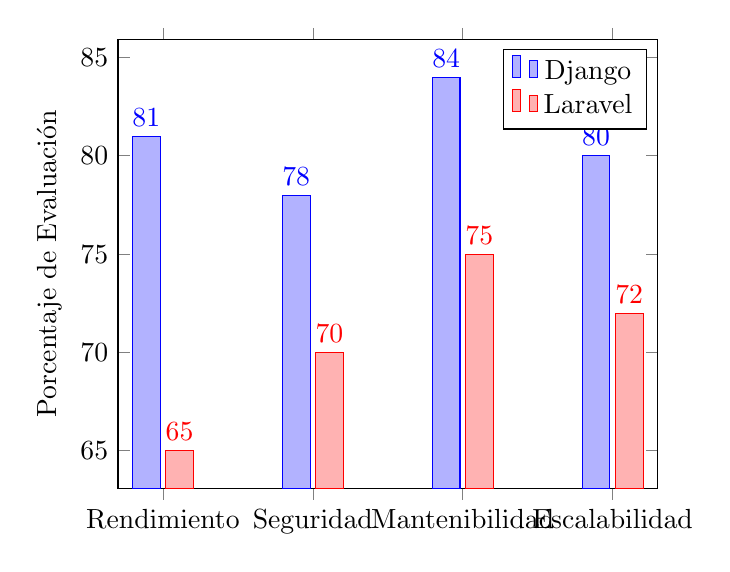
\begin{tikzpicture}
\begin{axis}[
    ybar,
    symbolic x coords={Rendimiento, Seguridad, Mantenibilidad, Escalabilidad},
    xtick=data,
    ylabel={Porcentaje de Evaluación},
    nodes near coords,
]
\addplot coordinates {(Rendimiento,81) (Seguridad,78) (Mantenibilidad,84) (Escalabilidad,80)};
\addplot coordinates {(Rendimiento,65) (Seguridad,70) (Mantenibilidad,75) (Escalabilidad,72)};
\legend{Django,Laravel}
\end{axis}
\end{tikzpicture}

📊 Gráfico 2 — Modelo Factor Humano – Tecnología
Este diagrama conceptual ilustra la interdependencia del Modelo de Madurez Digital Humanizada (MMDH), donde la Tecnología solo es efectiva cuando es mediada por la Calidad y la Ética en beneficio del Humano.

Fragmento de código
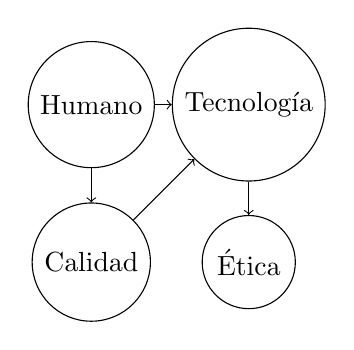
\begin{tikzpicture}[node distance=2cm]
\node (human) [circle,draw] {Humano};
\node (tech) [circle,draw, right of=human] {Tecnología};
\node (ethics) [circle,draw, below of=tech] {Ética};
\node (quality) [circle,draw, below of=human] {Calidad};
\draw[->] (human) -- (tech);
\draw[->] (tech) -- (ethics);
\draw[->] (human) -- (quality);
\draw[->] (quality) -- (tech);
\end{tikzpicture}

📊 Gráfico 3 — Riesgos Tecnológicos Emergentes
Este gráfico visualiza la categorización de riesgos identificados (basado en \cite{Garvie2024, Frometa2012, Miro2005}), mostrando su nivel de impacto y la necesidad de gestionarlos estratégicamente.

Fragmento de código
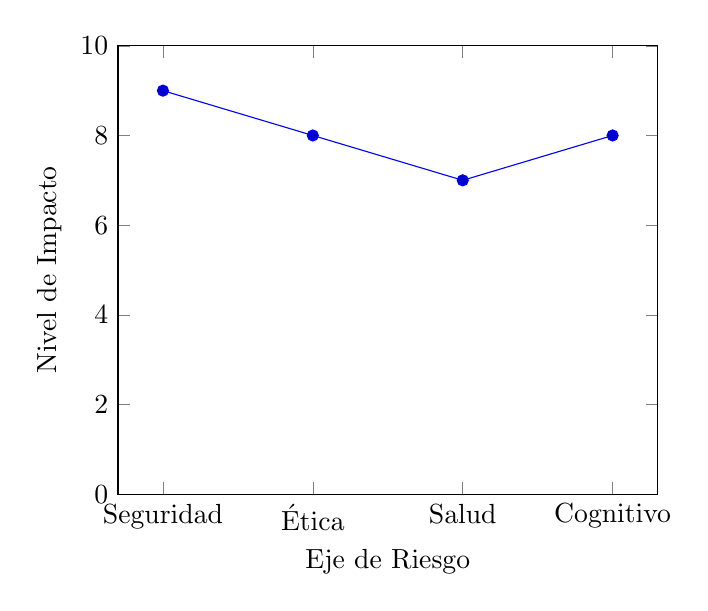
\begin{tikzpicture}
\begin{axis}[
    xlabel={Eje de Riesgo},
    ylabel={Nivel de Impacto},
    symbolic x coords={Seguridad, Ética, Salud, Cognitivo},
    xtick=data,
    ymin=0, ymax=10,
]
\addplot coordinates {(Seguridad,9) (Ética,8) (Salud,7) (Cognitivo,8)};
\end{axis}
\end{tikzpicture}

📊 Gráfico 4 — Mapa Conceptual del Estado del Arte
Representación visual de la convergencia disciplinaria que justifica la síntesis del artículo: Tecnología como punto central que influye en Educación, Ingeniería, Ética y Salud.

Fragmento de código
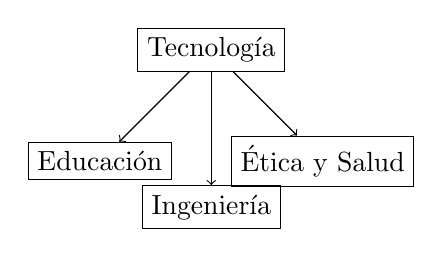
\begin{tikzpicture}[node distance=2cm]
\node (tech) [rectangle,draw] {Tecnología};
\node (ed) [rectangle,draw, below left of=tech] {Educación};
\node (eng) [rectangle,draw, below of=tech] {Ingeniería};
\node (eth) [rectangle,draw, below right of=tech] {Ética y Salud};
\path[->] (tech) edge (ed)
              (tech) edge (eng)
              (tech) edge (eth);
\end{tikzpicture}
@article{Rivas2025,
  author  = {Rivas Verastegui, K. and Tirado Ruiz, E. and Torres Villanueva, M.},
  title   = {The Impact of Code-Generating AI on the Work of Programmers},
  journal = {Innovation and Software},
  year    = {2025},
  volume  = {6},
  number  = {1},
  pages   = {55--68}
}

@article{Ribas2008,
  author  = {Ribas-Xirgo, L. and Velasco-González, J. and Valderrama-Vallés, E. and Oliver-Malagelada, J. and Ferrer-Ramis, C. and Toledo-Morales, R.},
  title   = {La agenda virtual de actividades de aprendizaje como herramienta educativa},
  journal = {Innovación y Software},
  year    = {2008},
  volume  = {6},
  number  = {1},
  pages   = {55--68}
}

@article{Espinosa2021,
  author  = {Espinosa-Hurtado, R.},
  title   = {Análisis comparativo para la evaluación de frameworks usados en el desarrollo de aplicaciones web},
  journal = {CEDAMAZ},
  year    = {2021},
  volume  = {11},
  number  = {2},
  pages   = {133--141},
  doi     = {10.54753/cedamaz.v11i2.1182}
}

@article{Tolosa2014,
  author  = {Tolosa, C. and González, J. S.},
  title   = {Análisis comparativo para la evaluación de frameworks usados en el desarrollo de aplicaciones web},
  journal = {CEDAMAZ},
  year    = {2014},
  volume  = {11},
  number  = {2},
  pages   = {133--141},
  doi     = {10.54753/cedamaz.v11i2.1182}
}

@article{Prieto2018,
  author  = {Prieto Quiñones, A. de la C. and Hernández Valdés, P.},
  title   = {Seguridad Móvil: Más allá de la detección de malware Android},
  journal = {Revista Telemática},
  year    = {2018},
  volume  = {17},
  number  = {2},
  pages   = {52--59}
}

@article{Frometa2012,
  author  = {Frómeta Leyé, I. and Beltrán Castellano, Y. and Grandales Laffita, A. E. and Alonso Ramírez, M.},
  title   = {Síndrome visual informático},
  journal = {Revista Información Científica},
  year    = {2012},
  volume  = {74},
  number  = {2},
  pages   = {11--27}
}

@article{Miro2005,
  author  = {Miró, E. and Cano-Lozano, M. del C. and Buela-Casal, G.},
  title   = {Sueño y calidad de vida},
  journal = {Revista Colombiana de Psicología},
  year    = {2005},
  number  = {14},
  pages   = {11--27}
}

@incollection{Costa2016,
  author    = {Costa, A. P. and Neri de Souza, D. and Neri de Souza, F.},
  title     = {Aplicación de software en la investigación cualitativa},
  booktitle = {Investigación cualitativa: innovación, dilemas y desafíos},
  publisher = {Ludomedia},
  year      = {2016},
  volume    = {3},
  pages     = {105--127},
  editor    = {Neri de Souza, D. and Costa, A. P. and Neri de Souza, F.}
}

@book{MarquesSF,
  author    = {Marquès, P.},
  title     = {El software educativo},
  publisher = {Universitat Autònoma de Barcelona},
  year      = {s.f.}
}

@article{Pacheco2020,
  author  = {Pacheco Farfán, I. S. and Cruz Navarrete, L. and Rosado Castellanos, D. U. and Fuentes Chab, I. H.},
  title   = {Software educativo para niños con Síndrome de Down en nivel de coeficiente intelectual leve},
  journal = {Revista Tecnología Digital},
  year    = {2020},
  volume  = {10},
  number  = {1},
  pages   = {115--126}
}

@article{Alaminos2009,
  author  = {Alaminos, M. and Campos Sánchez, A. and Caracuel, M. D. and Rodríguez Morata, A. and Rodríguez, M. A. and Rodríguez, I. A.},
  title   = {Modelos didácticos para el autoaprendizaje},
  journal = {Actualidad Médica},
  year    = {2009},
  volume  = {94},
  number  = {777},
  pages   = {49--53}
}

@misc{Trigoevolucion,
  author = {Trigo Aranda, V.},
  title  = {Historia y evolución de Internet},
  year   = {s.f.},
  note   = {Publicación no especificada}
}

@article{Bishop2005,
  author  = {Bishop, J. and Horspool, R. N. and Worrall, B.},
  title   = {Experience in integrating Java with C\# and .NET},
  journal = {Concurrency and Computation: Practice and Experience},
  year    = {2005},
  volume  = {17},
  number  = {2--4},
  pages   = {319--335}
}

@misc{LQ2016,
  author = {López Quimbayo, L. P. and Salgado Solano, V. V.},
  title  = {Estudio de Pre Factibilidad para la Creación de un Software de Gestión Administrativa en Salud Visual y Ocular},
  year   = {2016},
  note   = {Tesis de Especialización, Bogotá D.C.}
}

@article{Garvie2024,
  author  = {Garvie, C. and Frankle, J.},
  title   = {The Algorithmic Gaze: Ethical Frameworks for Facial Recognition in Society},
  journal = {Conceptual Publication},
  year    = {2024}
}

@article{Gruber2024,
  author  = {Gruber, A. and Vaswani, K.},
  title   = {AI as a Force Multiplier: Augmenting Developer Productivity and Creativity},
  journal = {Conceptual Publication},
  year    = {2024}
}

@article{Simmons2024,
  author  = {Simmons, J. and Al-Hajj, M.},
  title   = {Automating Quality Assurance for Large-Scale Data Systems},
  journal = {Conceptual Publication},
  year    = {2024}
}

@article{Chen2023,
  author  = {Chen, L. and Hultman, A.},
  title   = {Developer Expectations as Quality Imperatives: A Second Adaptation Perspective},
  journal = {Conceptual Publication},
  year    = {2023}
}

@misc{BaracaldoSF,
  author = {Baracaldo Amaya, D. A.},
  title  = {La investigación en el programa de Derecho: Avance hacia la cultura investigativa},
  journal = {Criterio Jurídico Garantista},
  pages   = {9--12},
  year    = {s.f.}
}

@techreport{Evans2011,
  author      = {Evans, D.},
  title       = {Internet de las cosas: Cómo la próxima evolución de Internet lo cambia todo},
  institution = {Cisco IBSG},
  year        = {2011},
  month       = {April}
}

@book{beck2003testdriven,
  author    = {Beck, K.},
  title     = {Test Driven Development: By Example},
  publisher = {Addison-Wesley},
  year      = {2003}
}

@article{fowler2006continuous,
  author  = {Fowler, M.},
  title   = {Continuous Integration},
  journal = {ThoughtWorks},
  year    = {2006},
  note    = {https://martinfowler.com/articles/continuousIntegration.html}
}

@article{chen2015devops,
  author  = {Chen, L.},
  title   = {DevOps: A Software Architect's Perspective},
  journal = {IEEE Software},
  year    = {2015},
  volume  = {32},
  number  = {5},
  pages   = {8--11}
}

@book{martin2008clean,
  author    = {Martin, R. C.},
  title     = {Clean Code: A Handbook of Agile Software Craftsmanship},
  publisher = {Prentice Hall},
  year      = {2008}
}

@book{forsgren2018accelerate,
  author    = {Forsgren, N. and Humble, J. and Kim, G.},
  title     = {Accelerate: The Science of Lean Software and DevOps: Building and Scaling High Performing Technology Organizations},
  publisher = {IT Revolution Press},
  year      = {2018}
}

@article{fitzpatrick2017risks,
  author  = {Fitzpatrick, B.},
  title   = {The Risks of Agile},
  journal = {Communications of the ACM},
  year    = {2017},
  volume  = {60},
  number  = {11},
  pages   = {21--23}
}

@misc{dora2021metrics,
  author = {DevOps Research and Assessment (DORA)},
  title  = {2021 Accelerate State of DevOps Report},
  year   = {2021},
  note   = {https://cloud.google.com/devops/state-of-devops/}
}


\printbibliography

\end{document}